\documentclass[9pt,twocolumn,twoside,printwatermark=false]{pinp}

%% Some pieces required from the pandoc template
\providecommand{\tightlist}{%
  \setlength{\itemsep}{0pt}\setlength{\parskip}{0pt}}

% Use the lineno option to display guide line numbers if required.
% Note that the use of elements such as single-column equations
% may affect the guide line number alignment.

\usepackage[T1]{fontenc}
\usepackage[utf8]{inputenc}

\definecolor{pinpblue}{HTML}{185FAF}  % imagecolorpicker on blue for new R logo
\definecolor{pnasbluetext}{RGB}{101,0,0} %


\newcommand{\TODO}{\marginnote{TODO}} \newcommand{\rlang}{\textit{R }} \newcommand{\rlangns}{\textit{R}} \newcommand{\slang}{\textit{S }} \newcommand{\rcpp}{\textit{Rcpp }} \newcommand{\rcppns}{\textit{Rcpp}} \newcommand{\clang}{\textit{C }} \newcommand{\clangns}{\textit{C}} \newcommand{\cpp}{\textit{C++ }} \newcommand{\cppns}{\textit{C++}} \newcommand{\fortran}{\textit{Fortran }} \newcommand{\fortranns}{\textit{Fortran}} \newcommand{\python}{\textit{Python}} \newcommand{\julia}{\textit{Julia}} \newcommand{\pkg}[1]{\textbf{#1}}

\title{Extending \rlang with C++:\\
A Brief Introduction to Rcpp}

\author[a]{Dirk Eddelbuettel}
\author[b]{James Joseph Balamuta}

  \affil[a]{Debian and R Projects; Chicago, IL, USA; \url{edd@debian.org}}
  \affil[b]{Depts of Informatics and Statistics, Univ. of Illinois at
Urbana-Champaign; Champaign, IL, USA; \url{balamut2@illinois.edu}}

\setcounter{secnumdepth}{0}

% Please give the surname of the lead author for the running footer
\leadauthor{Eddelbuettel and Balamuta}

% Keywords are not mandatory, but authors are strongly encouraged to provide them. If provided, please include two to five keywords, separated by the pipe symbol, e.g:
 \keywords{  applications and case studies |  statistical computing |  computationally intensive methods |  simulation  }  

\begin{abstract}
\rlang has always provided an application programming interface (API)
for extensions. Based on the \clang language, it uses a number of macros
and other low-level constructs
\end{abstract}

\dates{This version was compiled on \today}
\doi{\url{https://cran.r-project.org/package=Rcpp}}

\pinpfootercontents{Rcpp Vignette}

\begin{document}

% Optional adjustment to line up main text (after abstract) of first page with line numbers, when using both lineno and twocolumn options.
% You should only change this length when you've finalised the article contents.
\verticaladjustment{-2pt}

\maketitle
\thispagestyle{firststyle}
\ifthenelse{\boolean{shortarticle}}{\ifthenelse{\boolean{singlecolumn}}{\abscontentformatted}{\abscontent}}{}

% If your first paragraph (i.e. with the \dropcap) contains a list environment (quote, quotation, theorem, definition, enumerate, itemize...), the line after the list may have some extra indentation. If this is the case, add \parshape=0 to the end of the list environment.

\acknow{We thank Bob Rudis and Lionel Henry for excellent comments and
suggestion on an earlier}

\section{Introduction}\label{introduction}

The \rlang language and environment \citep{R:main} has established
itself as both an increasingly dominant facility for data analysis, and
the \emph{lingua franca} for statistical computing in both research and
application settings.

\subsection{Background}\label{background}

\begin{Shaded}
\begin{Highlighting}[]
\KeywordTok{library}\NormalTok{(}\StringTok{"Rcpp"}\NormalTok{)}
\KeywordTok{evalCpp}\NormalTok{(}\StringTok{"2 + 2"}\NormalTok{)}
\end{Highlighting}
\end{Shaded}

A graphical breakdown of all aspects of a corresponding \cpp function is
given in Figure \ref{fig:cpp-function-annotation}.

\begin{figure*}
  \begin{center}
    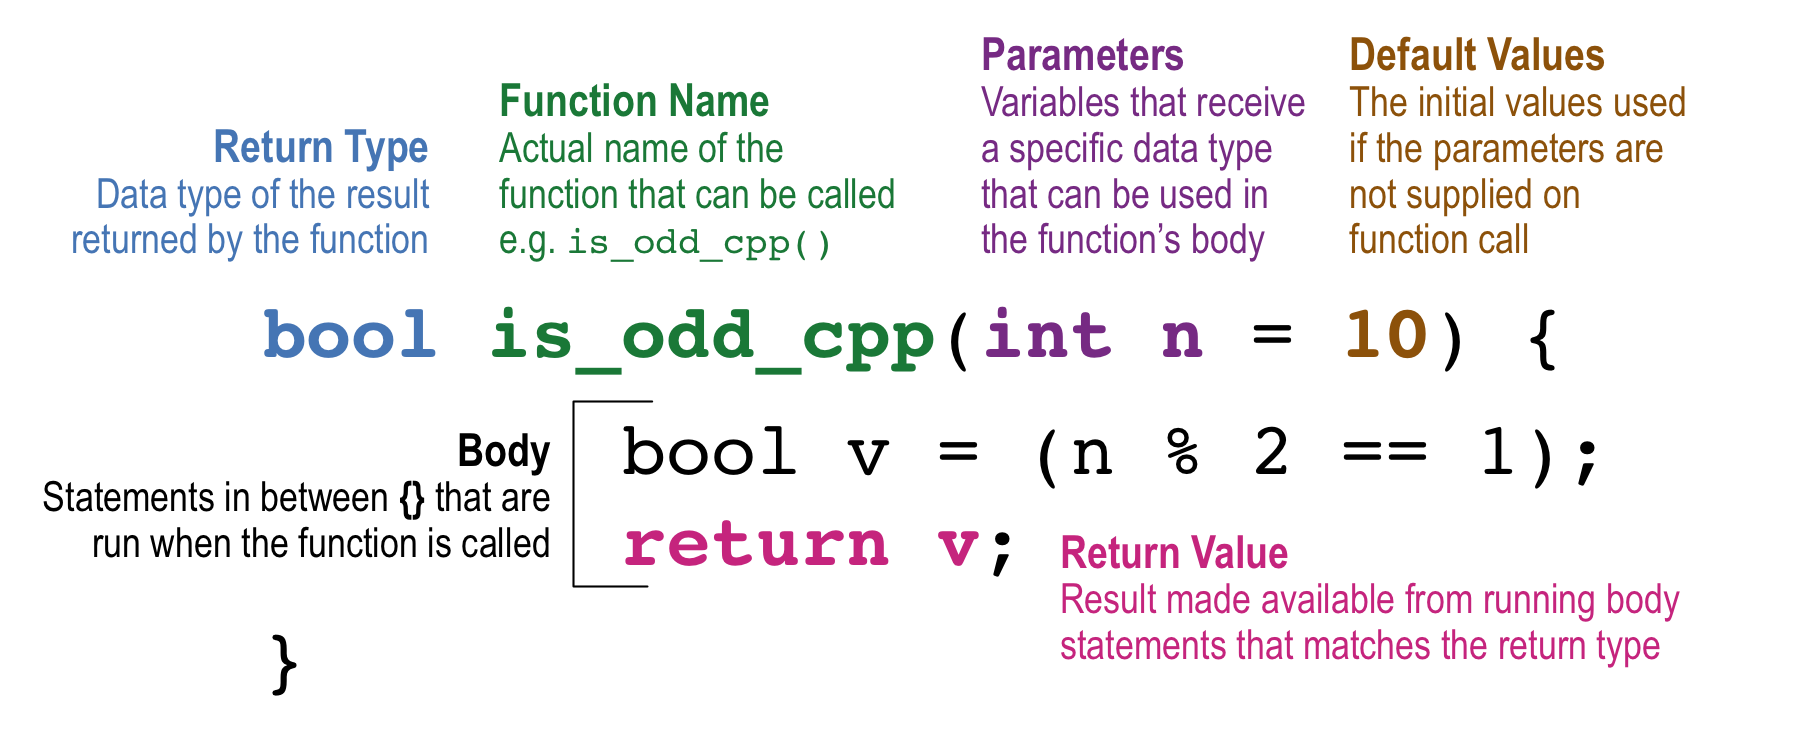
\includegraphics[width=5.5in]{figures/function_annotation_cpp.png}
    \caption{Graphical annotation of the \texttt{is\_odd\_cpp} function.}
    \label{fig:cpp-function-annotation}
  \end{center}
\end{figure*}

When using \rcppns, such \cpp functions can be directly embedded and
compiled in an \rlang
script file through the use of the \texttt{cppFunction()}

\section{Conclusion}\label{conclusion}

\rlang has always provided mechanisms to extend it. The bare-bones
\clang API is already used

%\showmatmethods
\showacknow

\pnasbreak 

\bibliography{Rcpp}
\bibliographystyle{jss}



\end{document}

